\input{header}

\AtBeginSubsection[]
{
	\begin{frame}<beamer>
		\frametitle{Outline}
		\tableofcontents[current,currentsubsection]
	\end{frame}
}

\begin{document}
\begin{frame}[allowframebreaks] \frametitle{Computability theory vs. complexity theory}
    \begin{itemize}
\item In Chapter 3 we showed that various TMs are equivalent
\item For example, single-tape and multi-tape TMs are equivalent
\item However, their ``time complexities'' are different
\end{itemize}\end{frame}

\begin{frame}[allowframebreaks] \frametitle{Complexity of Multi-tape
  TM}
  \begin{itemize}
  \item Theorem 7.8
    
  \item [] Let $t(n) \geq n$. For a $t(n)$ multi-tape TM

$\Rightarrow \exists$ equivalent 
$O(t(n)^2)$ single-tape TM
\item Idea for the proof: similar to how we proved their equivalence

\item We will show that simulating each step of a multi-tape TM
takes
$O(t(n))$ on a single-tape TM

\item Let $k$ be the number of tapes
\item How did we simulate a multi-tape TM?

  \begin{center}
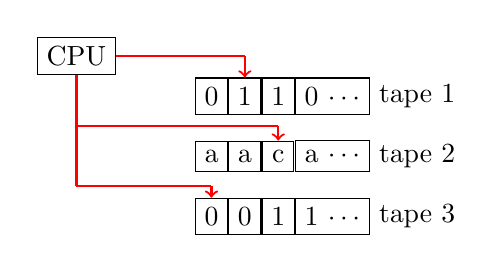
\begin{tikzpicture}[ampersand replacement=\&]
\matrix 
{
  \node[draw](0) {CPU}; \& [1cm]  \& \node(1){} ; \&\&\& \\
  \& \node[draw]{0}; \& \node[draw](a){1}; \& \node[draw]{1}; \& \node[draw]{0 $\cdots$};  \& \node{tape 1};\\
\node(2){} ; \&  \&  \& \node(21){} ; \&\& \\  
\& \node[draw]{a}; \& \node[draw]{a}; \& \node[draw](b){c}; \& \node[draw]{a $\cdots$}; \&  \node{tape 2}; \\
\node(3){} ; \& \node(31){} ; \&  \&  \&\& \\
\& \node[draw](c){0}; \& \node[draw]{0}; \& \node[draw]{1}; \& \node[draw]{1 $\cdots$}; \&  \node{tape 3}; \\
};

\draw [-,red,thick] (0) -- (1.center) ;
\draw [->,red,thick] (1.center) -- (a) ;
\draw [-,red,thick] (0) -- (2.center) ;
\draw [-,red,thick] (2.center) -- (21.center) ;
\draw [->,red,thick] (21.center) -- (b) ;
\draw [-,red,thick] (0) -- (3.center) ;
\draw [-,red,thick] (3.center) -- (31.center) ;
\draw [->,red,thick] (31.center) -- (c) ;
\end{tikzpicture}
\end{center}


\begin{center}
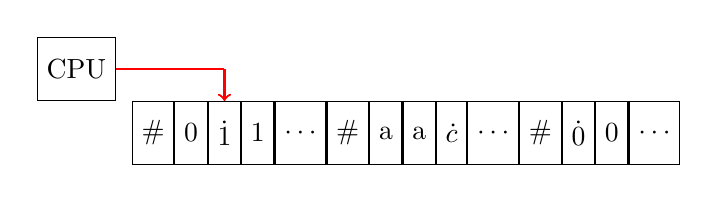
\begin{tikzpicture}[ampersand replacement=\&]
\matrix[nodes={minimum height=8mm}] 
{
  \node[draw](0) {CPU}; \& [0.2cm] \& \& \node(1){} ; \& \&\&\& \&\&\& \&\&\& \\
\& \node[draw]{\#};  \& \node[draw]{0}; \& \node[draw](a){$\dot{1}$}; \& \node[draw]{1}; \& \node[draw]{$\cdots$};
\& \node[draw]{\#};  \& \node[draw]{a}; \& \node[draw]{a}; \& \node[draw]{$\dot{\text{c}}$}; \& \node[draw]{$\cdots$}; 
\& \node[draw]{\#};  \& \node[draw](c){$\dot{0}$}; \& \node[draw]{0}; \& \node[draw]{$\cdots$}; \\
};

\draw [-,red,thick] (0) -- (1.center) ;
\draw [->,red,thick] (1.center) -- (a) ;
\end{tikzpicture}
\end{center}


\item To simulate each step of multi-tape TM, we scan to know where heads point to
  and do the update
\item However, we may have to
right shift the tape 
\item So we need to know the tape length. It is
\begin{equation*}
  k \times O(t(n)) = O(t(n)) 
\end{equation*}
  
\item Note that each tape of multi-tape TM has $O(t(n))$ length. Why?

\item A $t(n)$ multi-tape TM generates
$O(t(n))$ contents in 
$O(t(n))$ time

\item Thus the cost of
  simulating each step of multi-tape TM on a single-tape TM is
  $O(t(n))$
\item There are $O(t(n))$ multi-tape TM steps, so
  the total cost is
  \begin{equation*}
    O(t(n)) \times O(t(n)) = O(t(n)^2)
\end{equation*}
\end{itemize}\end{frame}

\begin{frame}[allowframebreaks] \frametitle{Complexity of Nondeterministic TM}
  \begin{itemize}
\item Remember NTM is a decider if all branches halt on all inputs

\item Definition of NTM time complexity $t(n)$:

\item [] maximum \# of steps the machine uses for any path from root
  to a leave

\item Theorem 7.11
\item [] Let $t(n) \geq n$. For a $t(n)$ NTM (single tape)

\item [] $\Rightarrow \exists \text{ a } 2^{O(t(n))}$ TM (single tape)
\item Assume $b$ is the maximal number of branches at each layer
\item Recall our way of doing the simulation is by the following
  three-tape TM

\begin{center}
  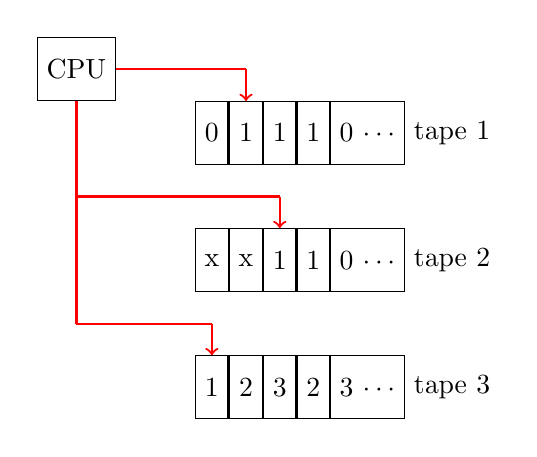
\begin{tikzpicture}[ampersand replacement=\&]
\matrix[nodes={minimum height=8mm}]     
{
  \node[draw](0) {CPU}; \& [1cm]  \& \node(1){} ; \&\&\& \& \\
  \& \node[draw]{0}; \& \node[draw](a){1}; \& \node[draw]{1}; \& \node[draw]{1};  \& \node[draw]{0 $\cdots$};  \& \node{tape 1};\\
\node(2){} ; \&  \&  \& \node(21){} ; \&\& \&\\  
\& \node[draw]{x}; \& \node[draw]{x}; \& \node[draw](b){1}; \& \node[draw]{1}; \& \node[draw]{0 $\cdots$}; \& \node{tape 2};  \\
\node(3){} ; \& \node(31){} ; \&  \&\& \& \&\\
\& \node[draw](c){1}; \& \node[draw]{2}; \& \node[draw]{3}; \& \node[draw]{2}; \& \node[draw]{3 $\cdots$}; \&  \node{tape 3}; \\
};

\draw [-,red,thick] (0) -- (1.center) ;
\draw [->,red,thick] (1.center) -- (a) ;
\draw [-,red,thick] (0) -- (2.center) ;
\draw [-,red,thick] (2.center) -- (21.center) ;
\draw [->,red,thick] (21.center) -- (b) ;
\draw [-,red,thick] (0) -- (3.center) ;
\draw [-,red,thick] (3.center) -- (31.center) ;
\draw [->,red,thick] (31.center) -- (c) ;
\end{tikzpicture}
\end{center}

\item We use a depth-first way for the simulation
\item That is, after one layer is finished, we do the next

\item Tape 3: all possible paths so far

\item Total number of nodes in the tree:
\begin{equation*}
  O(b^{t(n)})
\end{equation*}

\item Tape 2: run the original input $w$ from root to one node in the
  tree

\item Cost of running from root to one node in tape 2: $O(t(n))$

\item Update of tape 3: $O(b^{(t(n))})$

\item Total cost $\leq O(b^{t(n)})$ for each node
\item Total time:
  \begin{equation*}
    \begin{split}
& \# \text{ nodes } \times \text{ cost per node}\\      
= &   O(b^{t(n)}) \times O(b^{t(n)}) \\
= & O((b^2)^{t(n)} ) = 2^{O(t(n))}
\end{split}
\end{equation*}
\item Note that in the above equality we used
  \begin{equation*}
    b^{t(n)} \times b^{t(n)}
    = b^{2t(n)} =
    2^{\log_2 b^{2t(n)}} = 2^{(\log_2 b)(2 t(n))}
  \end{equation*}

\item This is by a 3-tape TM
\item To use a single-tape TM to simulate a 3-tape one, we need
  \begin{equation*}
(2^{O(t(n))})^2
= 2^{O(t(n))}
\end{equation*}
cost because
\begin{equation*}
  (2^{O(t(n))})^2
\leq (2^{ct(n)})^2
= 2^{2ct(n)} 
= 2^{O(t(n))}
\end{equation*}
\end{itemize}\end{frame}

\end{document}
